%%
%\subsection{Perpendicular Bisectors}
\renewcommand{\theequation}{\theenumi}
\begin{enumerate}[label=\arabic*.,ref=\thesubsection.\theenumi]
\numberwithin{equation}{enumi}

\item Show that $\cos 2A = 1 -\sin^2 A$.
\\
\solution In $\triangle OBC$, using the cosine formula, 
\begin{align}
\cos 2A = \frac{R^2+R^2 - a^2}{2R^2} = 1 -\frac{a^2}{2R^2}
\label{eq:crad_cos2a}
\end{align}
%
Using the sine formula, 
\begin{align}
\frac{\sin 2A}{a} &= \frac{\sin \theta_1}{R} = \frac{\sin\brak{90\degree- A}}{R}
\\
\implies \sin 2A &= \frac{a\cos A}{R}
\label{eq:crad_sin2a}
\end{align}
%
from \eqref{eq:tri_ccentre_A1} and \eqref{eq:tri_baudh_comp}.	Using \eqref{eq:tri_sin_cos_id}, 
\begin{align}
\cos^2 2A + \sin^2 2A&= 1
\\
\implies \brak{1 -\frac{a^2}{2R^2}}^2 + \brak{\frac{a\cos A}{R}}^2 &= 1
\\
\implies 
\end{align}
%
upon substituting from \eqref{eq:crad_cos2a}  and \eqref{eq:crad_sin2a}.



%\item Draw $OD \perp BC$, where $\vec{D}$  lies on $BC$.
%\\
%\solution
%A circle with centre $\vec{O}$ can be drawn through $\vec{A}, \vec{B}, \vec{C}$.  This circle is known as the {\em circumcircle}.  
%
%\item
%	In Fig. \ref{fig:tri_geo_ccentre}, $OE \perp AC, OF \perp AB, AE=EC, AF=FB$.  $OE$ and $OF$ are known as the {\em perpendicular bisectors} of $AC$ and $AB$ respectively.  Show that $OA=OB=OC$.
%%
%\\
%\solution Using SAS, $\triangle OEA \cong \triangle OEC$.  Thus, $OA = OC$.  Similarly,   $\triangle OFA \cong \triangle OFB \implies OA = OB$.
%
%\item
%	In Fig. \ref{fig:tri_geo_ccentre}, show that if $OD \perp BC$, $BD=DC$, i.e., $OD$ is the perpendicular bisector of $BC$.
%.
%\\
%\solution $\because OB = OC$, using RHS congruence, $\triangle ODC \cong \triangle ODB$.  Hence $BD = DC$.\item
%	In Fig. \ref{fig:tri_geo_ccentre}, show that if $BD=DC$, $OD \perp BC$.
%.
%\\
%\solution Use SSS.
%%%
%%%
%\begin{figure}[!ht]
%	\begin{center}
%		
%%		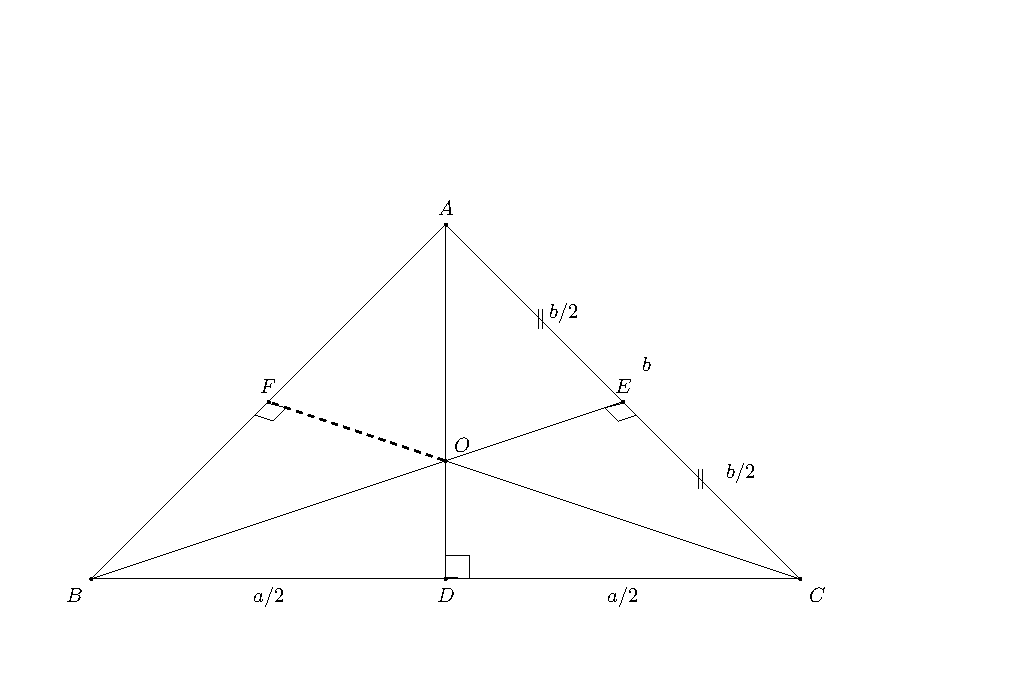
\includegraphics[width=\columnwidth]{./figs/fig_3.8.eps}
%		\resizebox{\columnwidth}{!}{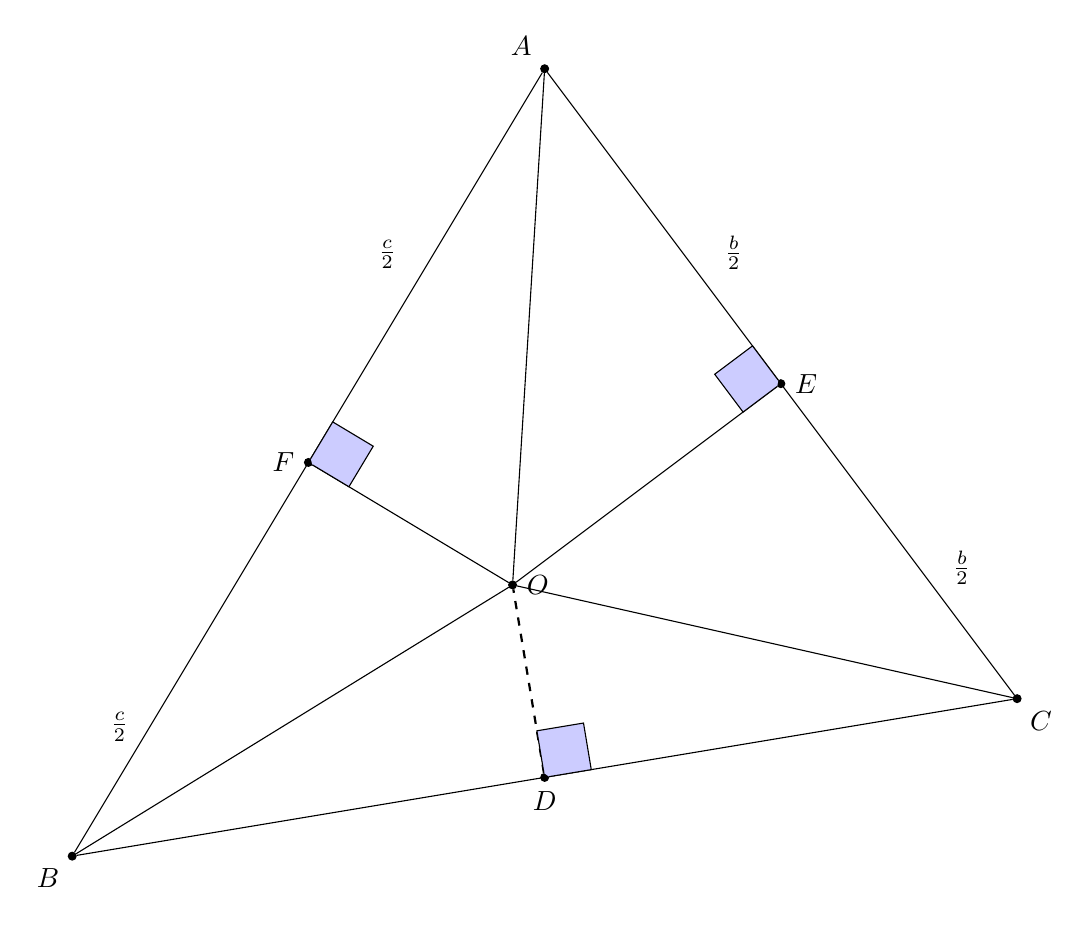
\begin{tikzpicture}
[
 scale=2,
  >=stealth,
  point/.style = {draw, circle, fill = black, inner sep = 1pt},
]
\node (B) at (-2,-2)[point,label = below left:${B}$] {};
\node (A) at (1,3)[point,label = above left:${A}$] {};
\node (C) at (4,-1)[point,label = below right:${C}$] {};
\draw (A) -- (B) -- (C) -- (A);

\node (D) at (1,-1.5)[point,label = below:$D$] {};

\node (F) at (-0.5,0.5)[point,label = left:$F$] {};

\node (E) at (2.5,1)[point,label = right:$E$] {};

\node (O) at (0.7962963,-0.27777778) [point,label = right:$O$] {};

\draw[thick, dashed] (D) -- (O);
\draw (F) -- (O);
\draw (E) -- (O);
\draw (A) -- (O);
\draw (B) -- (O);
\draw (C) -- (O);

\tkzMarkRightAngle[fill=blue!20,size=.3](A,E,O)
\tkzMarkRightAngle[fill=blue!20,size=.3](A,F,O)
\tkzMarkRightAngle[fill=blue!20,size=.3](O,D,C)


\node [below] at (3.65,0) {\strut $\frac{b}{2}$};
\node [below] at (2.2,2) {\strut  $\frac{b}{2}$};


%\node [below] at (2.5,-1.2) {\strut a/2};    
%\node [below] at (0,-1.65) {\strut a/2};  
      
\node [below] at (-1.7,-1) {\strut  $\frac{c}{2}$}; 
\node [below] at (0,2) {\strut  $\frac{c}{2}$};   


\end{tikzpicture}
}
%%		\includegraphics[width=\columnwidth]{./figs/fig26_def}
%		%\vspace*{-10cm}
%%		\resizebox{\columnwidth}{!}{\documentclass{standalone}
\usepackage{tikz}
\usepackage{tkz-euclide}
\usetkzobj{all}
%\usepackage{amsmath}
\providecommand{\brak}[1]{\ensuremath{\left(#1\right)}}

\begin{document}
\begin{tikzpicture}
[scale=2,>=stealth,point/.style={draw,circle,fill = black,inner sep=0.5pt},]

\node (E) at (1.5, 1.5)[point,label=above :$E$] {};
\node (F) at (-1.5, 1.5)[point,label=above :$F$] {};
\node (A) at (0, 3)[point,label=above :$A$]{};
\node (B) at (-3, 0)[point,label=below left:$B$]{};
\node (C) at (3, 0)[point,label=below right:$C$]{};
\node (D) at (0,0)[point,label=below :$D$] {};
\node (O) at (0,1)[point,label=above right :$O$] {};


\draw (B)--(A);
\draw (A)--(C);
\draw (B)--(C);
\draw (B)--(E);
\draw (C)--(O);
\draw (A)--(D);
\draw [thick,dashed] (O) -- (F);

\node [above] at (1.7,1.7) {$b$};
\node [above] at (2.5,.75) {$b/2$};
\node [above] at (1,2.1) {$b/2$};
\node [above] at (-1.5,-0.3){$a/2$};
\node [above] at (1.5,-0.3){$a/2$};
\tkzMarkRightAngle[size=.16](B,F,O)
\tkzMarkRightAngle[size=.16](C,E,O)
\tkzMarkRightAngle[size=.2](A,D,C)
\draw   -- (4.3,1.7) node[midway] {$\parallel$};
\draw   -- (1.6,4.4) node[midway] {$\parallel$};

\end{tikzpicture}
\end{document}}
%	\end{center}
%	\caption{Perpendicular bisectors meet at a point}
%	\label{fig:tri_geo_ccentre}	
%\end{figure}
%%
%%\solution In $\triangle$s $ODB$ and $ODC$, using Budhayana's theorem,
%%%
%%\begin{equation}
%%\begin{split}
%%OB^2 &= OD^2 + BD^2 \\
%%OC^2 &= OD^2 + DC^2 
%%\end{split}
%%\end{equation}
%%
%%Since $BD = DC = \frac{a}{2}$, $OB = OC$.  Similarly, it can be shown that $OA = OC$.  Thus, $OA=OB=OC$.
%%
%\item
%	In $\triangle AOB$, $OA = OB$.  Such a triangle is known as an isoceles triangle.
%%
%%\item
%%	Show that $AF = BF$.
%%
%%\solution Trivial using Budhayana's theorem.  This shows that $OF$ is a perpendicular bisector of $AB$. 
%\\
%{\em Conclusion:}  The perpendicular bisectors of a triangle meet at a point.
%%
%\item In Fig. \eqref{fig:tri_geo_ccentre_circ}, $OA = OB=OC = R$.  Show that $\angle BOC = 2\angle BAC$. 			\label{ch4_prob_circle_subtend}
%
%\begin{figure}[!ht]
%	\begin{center}
%		
%		\resizebox{\columnwidth}{!}{\begin{tikzpicture}
[
 scale=2,
  >=stealth,
  point/.style = {draw, circle, fill = black, inner sep = 1pt},
]
\node (B) at (-2,-2)[point,label = below left:${B}$] {};
\node (M) at (0.71741199, -1.547098)[point,label = below left:${M}$] {};
\node (A) at (1,3)[point,label = above left:${A}$] {};
\node (C) at (4,-1)[point,label = below right:${C}$] {};
\draw (A) -- (B) -- (C) -- (A);

\node (D) at (1,-1.5)[point,label = below:$D$] {};

\node (F) at (-0.5,0.5)[point,label = left:$F$] {};

\node (E) at (2.5,1)[point,label = right:$E$] {};

\node (O) at (0.7962963,-0.27777778) [point,label = above right:$O$] {};

%\draw[thick, dashed] (D) -- (O);
\draw[thick, dashed] (M) -- (O);
%\draw (F) -- (O);
%\draw (E) -- (O);
\draw (A) -- (O);
\draw (B) -- (O);
\draw (C) -- (O);

\tkzMarkAngle[size=0.3](M,O,C)
\tkzMarkAngle[size=0.35](B,O,M)
\tkzMarkAngle[size=0.3](O,A,C)
\tkzMarkAngle[size=0.35](B,A,O)
\tkzMarkAngle[size=0.3](A,C,O)
\tkzMarkAngle[size=0.3](O,B,A)

\draw ($(A) + (0.2,-0.5)$) node{$\theta_1$};
\draw ($(A) + (-0.2,-0.5)$) node{$\theta_2$};
\draw ($(B) + (0.5,0.5)$) node{$\theta_2$};
\draw ($(C) + (-0.5,0.4)$) node{$\theta_1$};
\node [above] at ($ (O)!0.5!(C) $){$R$};
\node [above] at ($ (O)!0.5!(B) $){$R$};
\node [right] at ($ (O)!0.5!(A) $){$R$};
\draw ($(O) + (0.2,-0.5)$) node{$\alpha$};
\draw ($(O) + (-0.3,-0.5)$) node{$\beta$};
%\node [above] at (-0.2,-0.5){$\alpha$};
%\node [above] at (0.2,-0.6){$\beta$};

%\tkzMarkRightAngle[fill=blue!20,size=.3](A,E,O)
%\tkzMarkRightAngle[fill=blue!20,size=.3](A,F,O)
%\tkzMarkRightAngle[fill=blue!20,size=.3](O,D,C)


%\node [below] at (3.65,0) {\strut $\frac{b}{2}$};
%\node [below] at (2.2,2) {\strut  $\frac{b}{2}$};


%\node [below] at (2.5,-1.2) {\strut a/2};    
%\node [below] at (0,-1.65) {\strut a/2};  
      
%\node [below] at (-1.7,-1) {\strut  $\frac{c}{2}$}; 
%\node [below] at (0,2) {\strut  $\frac{c}{2}$};   


\end{tikzpicture}
}
%	\end{center}
%	\caption{$\angle BOC = 2\angle BAC$}
%	\label{fig:tri_geo_ccentre_circ}	
%\end{figure}
%%
%\solution Note that $\alpha$ and $\beta $ are exterior angles for $\triangle$s $AOB$ and $AOC$, which are isosceles.
%%
%\item Show that 
%\begin{align}
%\label{eq:tang_eq}
%\begin{split}
%AE=AF
%\\
%BD = BF
%\\
%CD = CE
%\end{split}
%\end{align}
%%
%\solution $\because$
%\begin{align}
%%\label{eq:tang_eq}
%BD = OB \cos \frac{B}{2}
%\\
%BF = OB \cos \frac{B}{2}
%\end{align}
%in right $\triangle$s $OBD$ and $OBE$, \eqref{eq:tang_eq} is obtained.
%
%\item Find $R$ in terms of $a, b, c$.
\end{enumerate}

